In the following sections we divide our analysis into three sections: 
Affinity filtering Analysis, Interaction Analysis and Activity Analysis
\subsection{Affinity filtering}
Affinity filtering is based on the idea that affinity between users expressed in social networks via interactions and activities is predictive 
of user preferences. Figure \ref{Fig1} compares the accuracies of constant predictor and social matchbox with affinity filtering (naive bayes,
logistic regression and SVM) for interaction and activity (group, page, favourite) features. 

In all of our experiments Affinity filtering performed significantly better than Social Matchbox and constant predictor except for the naive bayes.
Naive bayes performed comparatively worse than Logistic regression and SVM counterpart. It's  due to the correlation between features which is contrary to the
conditional independance assumption made by naive bayes model.

Also, Figure \ref{Fig1} shows that activities are more predictive than interactions. Among the activities, page likes are the most predictive followed by group
membership and favourites.

\subsection{Interaction Analysis}
In figure \ref{Fig2} we plot conditional entropy of modality and action for incoming/outgoing interactions constrained to the link liked by atleast k friends.
Figure \ref{Fig2} shows that 
\begin{itemize}
  \item Some interactions are more predictive than other. For eg. videos and photo interactions were found to be significantly more predictive than post
  		and link interactions. Similarly, tagging action is often more predictive than commenting and liking. 
  \item As noted by previous work~\cite{saez2011high}, we observe that outgoing interactions are more predictive than incoming interactions. Furthermore, the differentiation between 
  		predictiveness modalities and actions is more pronounced in outgoing interactions than in incoming interactions.
  \item It shows that the conditional entropy decreases as the number of friends liking the link increases.
        It suggests that the discriminitivenes of interaction social affinity features increases as more friend like the item.   
  \end{itemize}

\subsection{Activity Analysis}
In this section we evaluate the correlation between the conditional entropy and size of groups, pages and favourites. 
\begin{itemize}
  \item Fig \ref{Fig3} shows the relationship between conditional entropy/logistic regression weights and size of activity groups. It  shows that the activity groups
  	    of small size can be highly predictive whereas large groups are rarely predictive.
  \item In \ref{Fig4} we plot the average conditional entropy of top 10\% features cumulative over the size of activity group. It distinctly shows that the small sized
  		group, pages and favourites have low average conditional entropy. Furthermore, it explains average conditional entropy decreases as size increases. From the 
  		figure \ref{Fig4} we can infer that the group size upto 50 and page/favourite size upto $10^{5}$ can be highly predictive.   
  \item We also analyze predictiveness of favourites by categories in fig \ref{Fig5}. It shows that television, books, music and movies are predictive whereas 
  favourite teams, sports and athletes are less predictive. 
\end{itemize}

\begin{figure*}[t!]
\centering
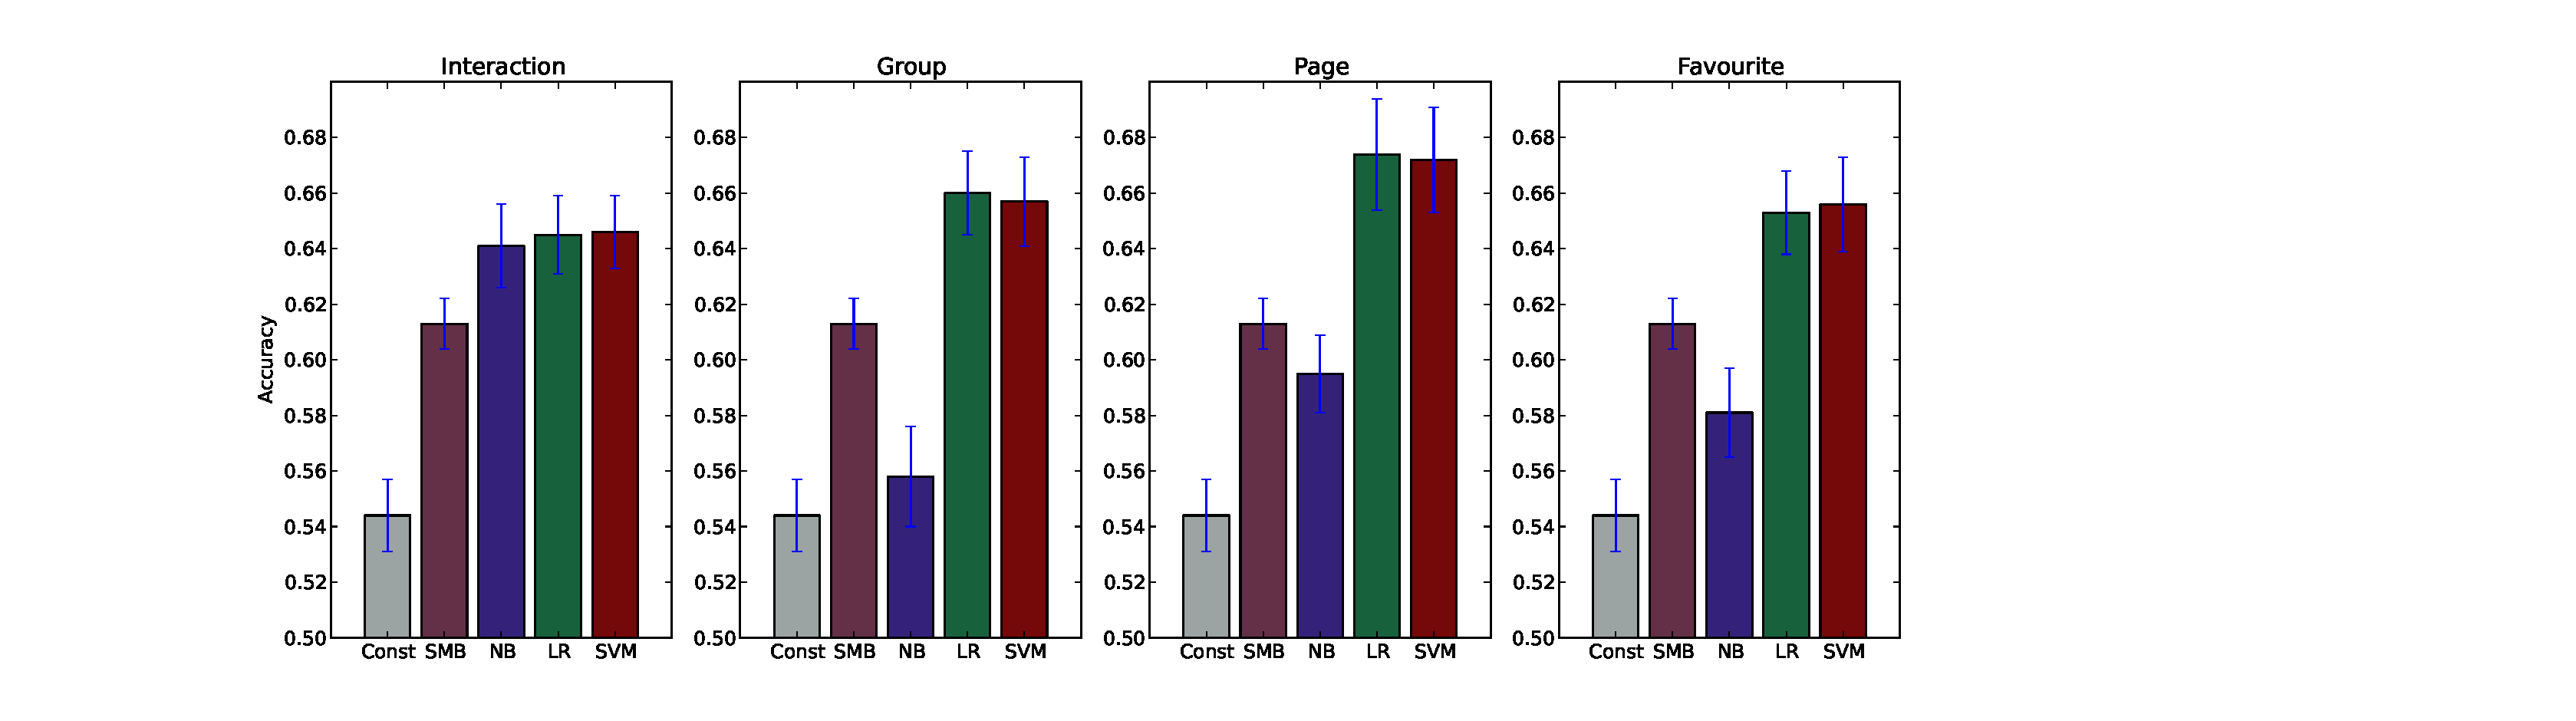
\includegraphics[width=230mm, height=50mm]{data/plots/accuracy/accuracy.eps}
\caption{ Accuracy of predictors (constant, social matchbox, naive bayes, logistic regression, SVM) for Interaction and Activity  features }
\label{Fig1}
\end{figure*}

\begin{figure*}
\centering
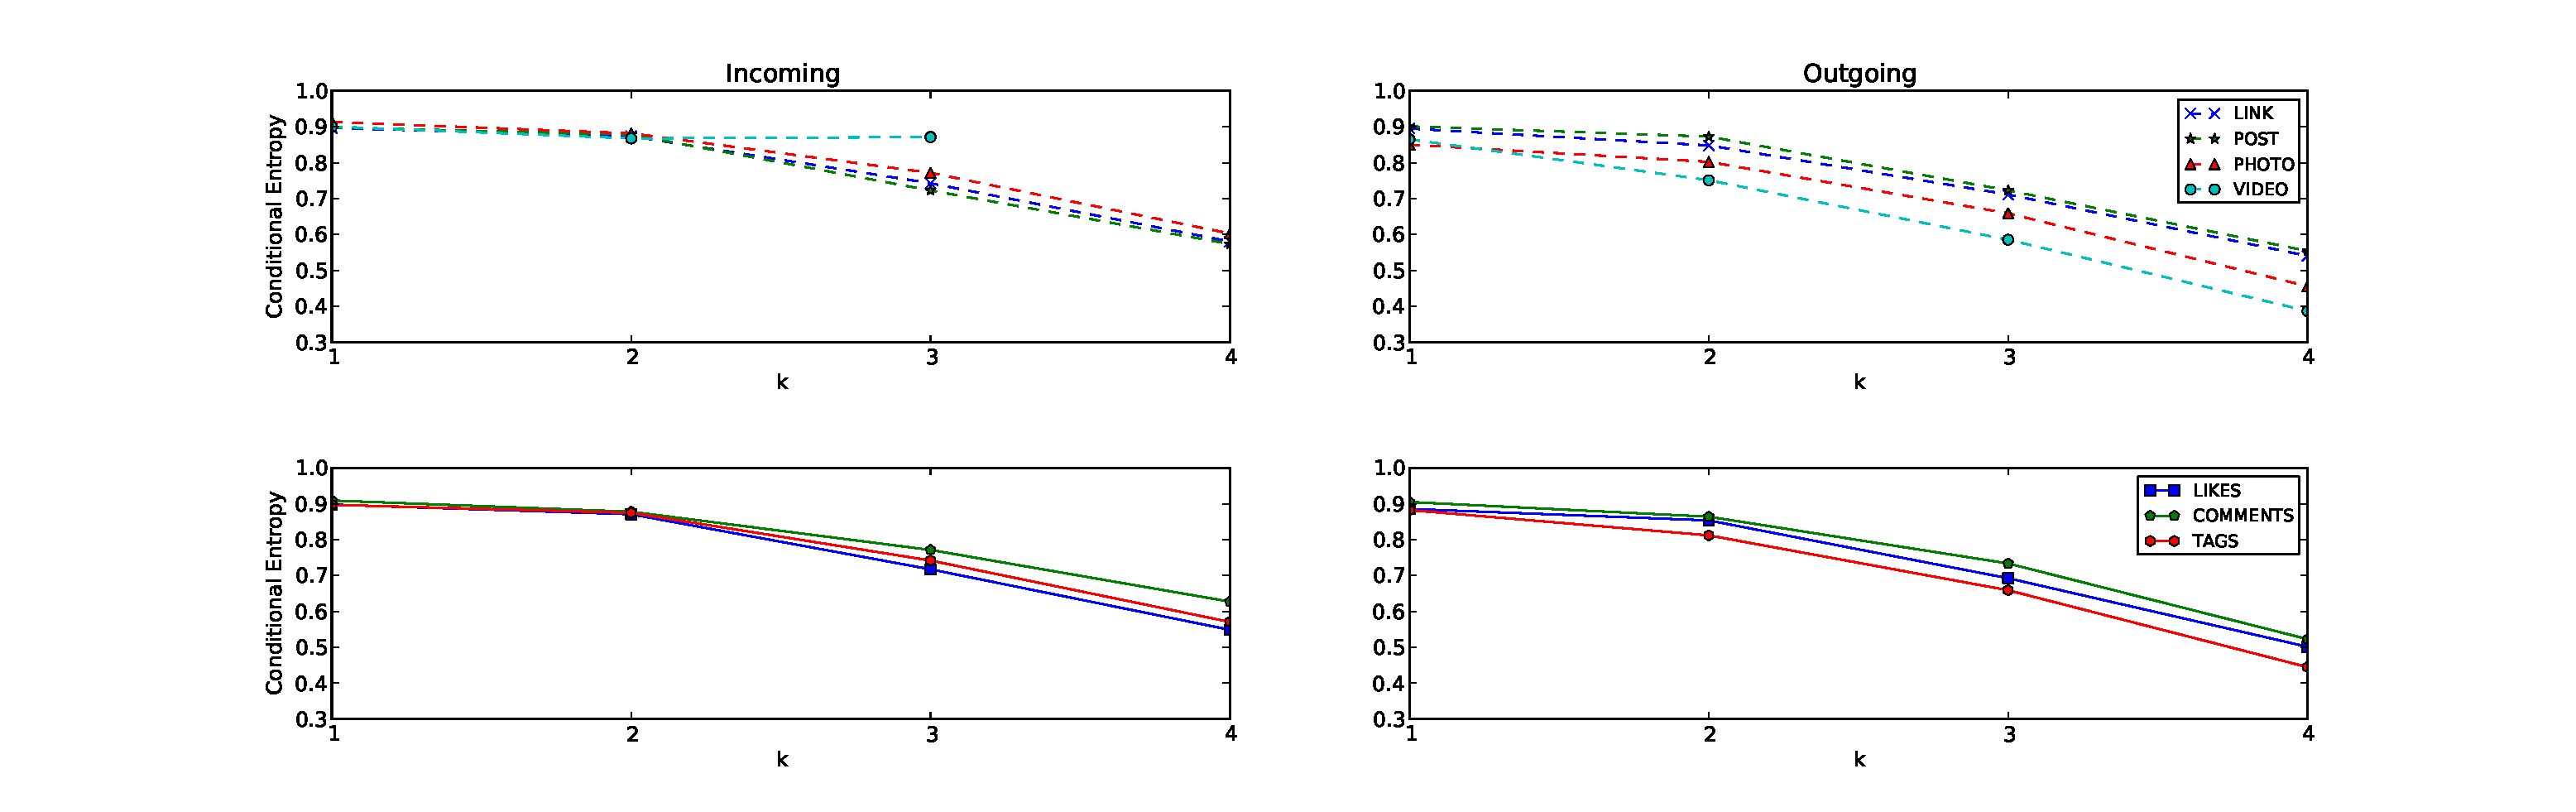
\includegraphics[width=160mm, height=40mm]{data/plots/vsk/ModalityActionsvsKFriends.eps}
\caption{Conditional Entropy  of modalities/activities for incoming/outgoing interactions vs item liked by atleast k friends}
\label{Fig2}
\end{figure*}

\begin{figure*}[h]
\centering
\begin{tabular}{ccc}
\subfloat[Fig:][]{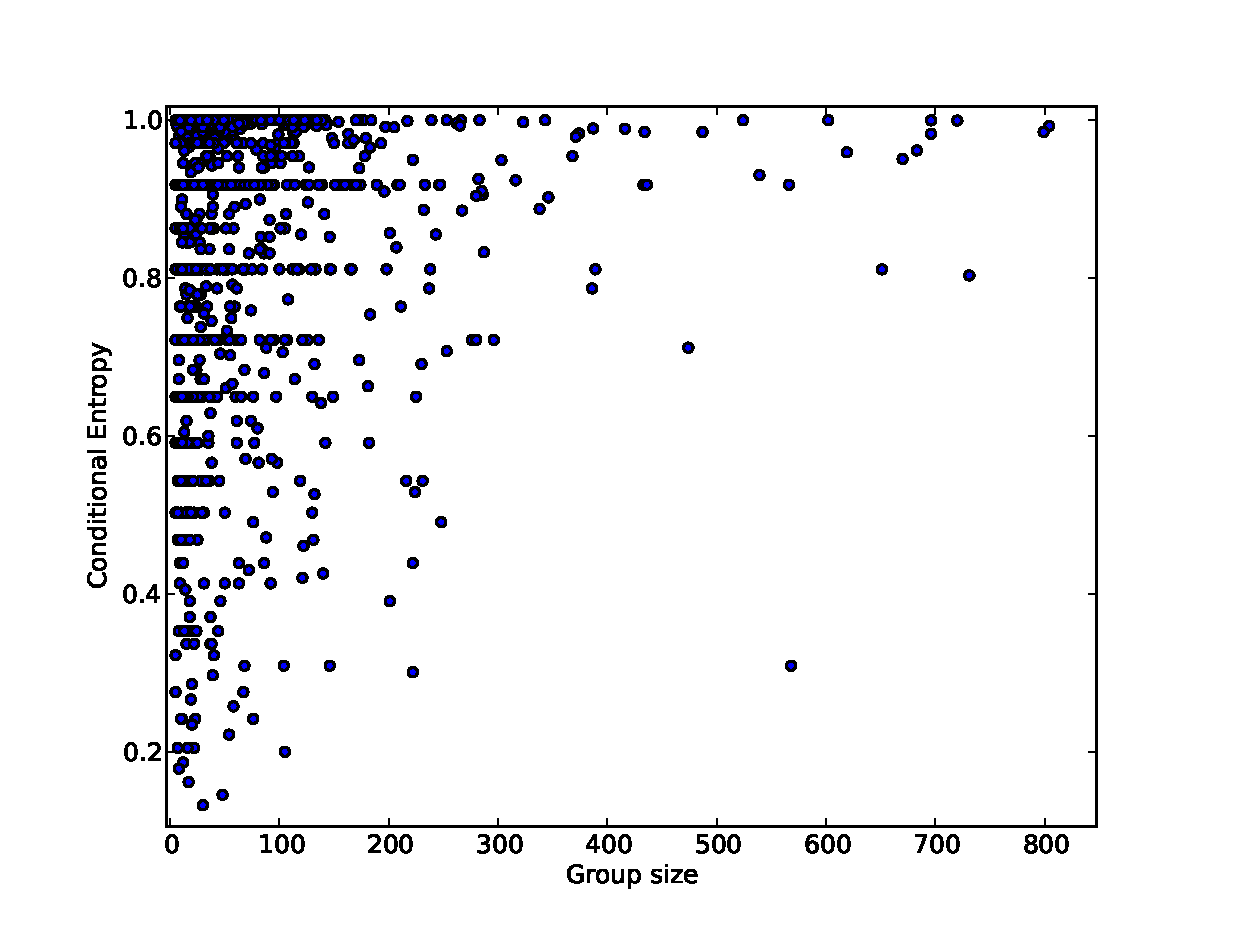
\includegraphics[width=40mm, height=25mm]{data/plots/scatterplots/vssize/CEvsGroupSize.eps}}
\subfloat[Fig:][]{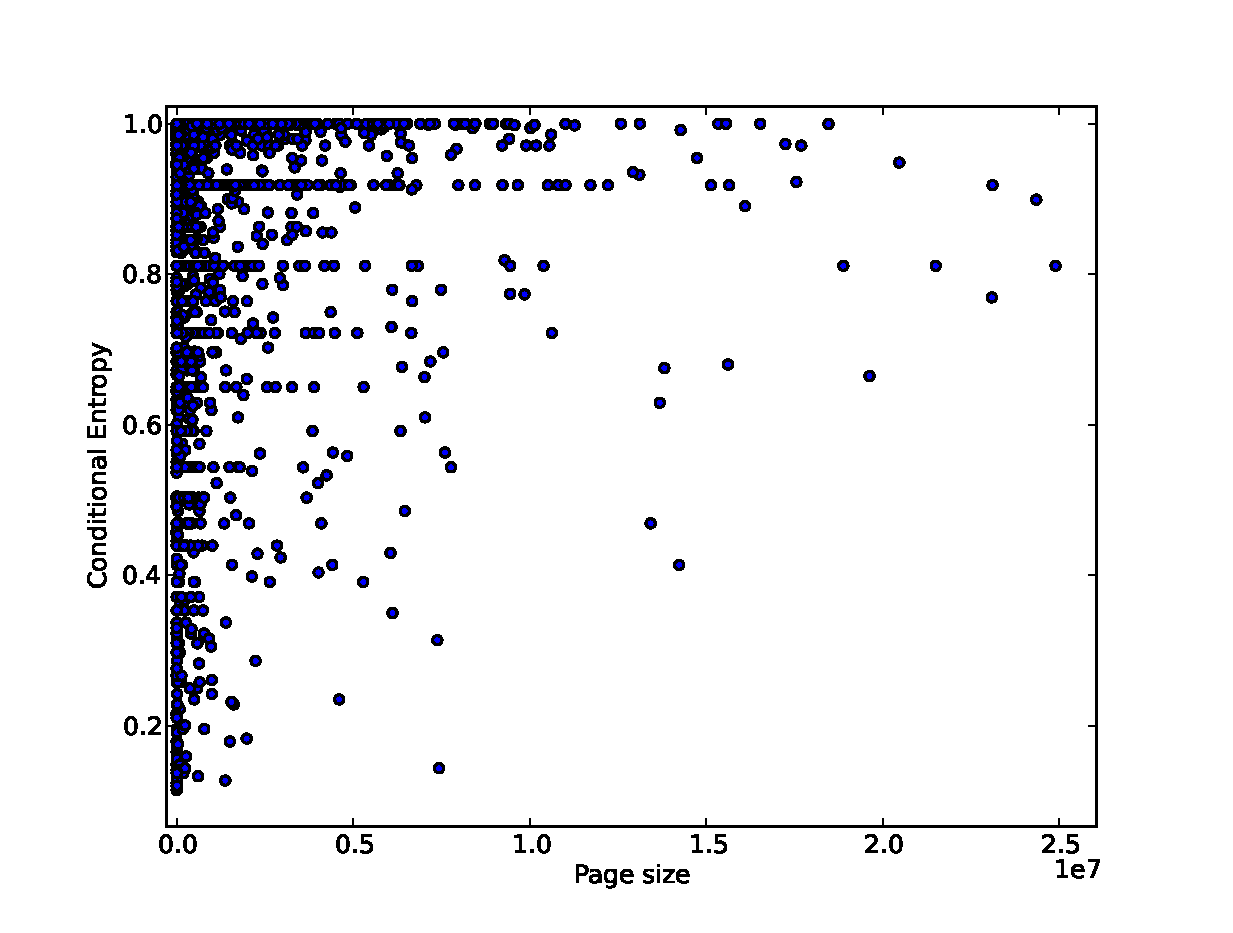
\includegraphics[width=40mm, height=25mm]{data/plots/scatterplots/vssize/CEvsPageSize.eps}}
\subfloat[Fig:][]{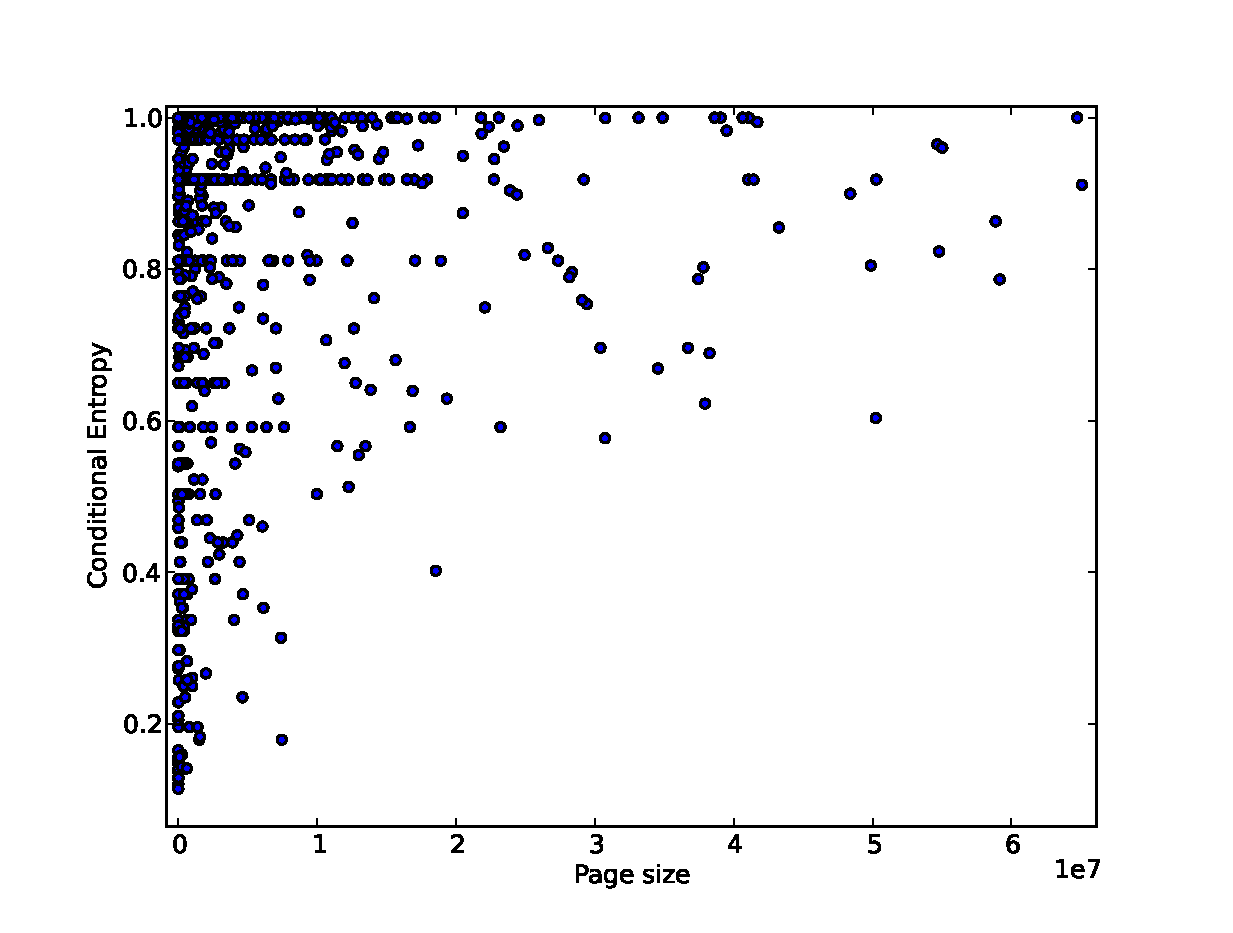
\includegraphics[width=40mm, height=25mm]{data/plots/scatterplots/vssize/CEvsFavSize.eps}} \\
\subfloat[Fig:][]{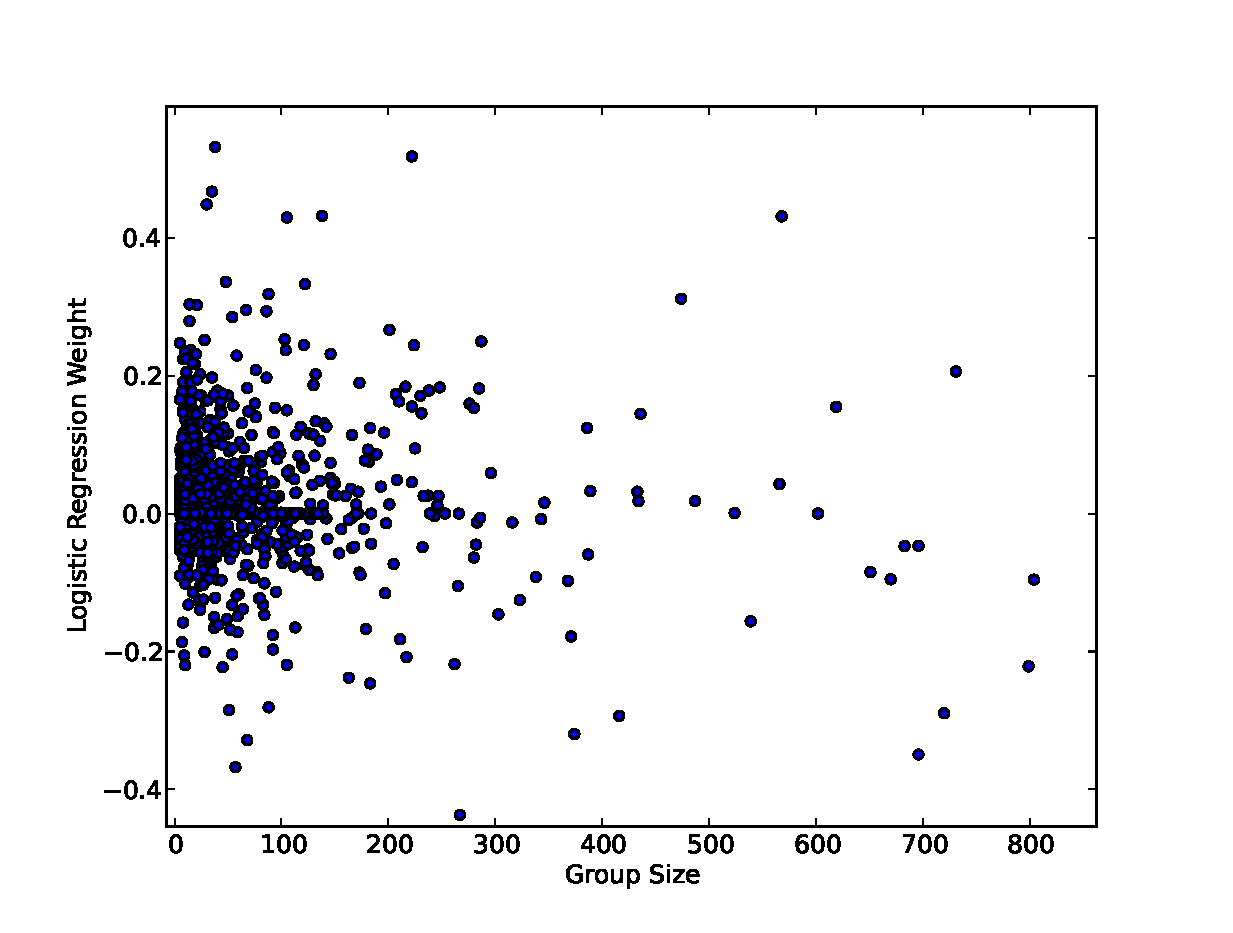
\includegraphics[width=40mm, height=25mm]{data/plots/scatterplots/LRweights/LRweightvsGroupSize.eps}}
\subfloat[Fig:][]{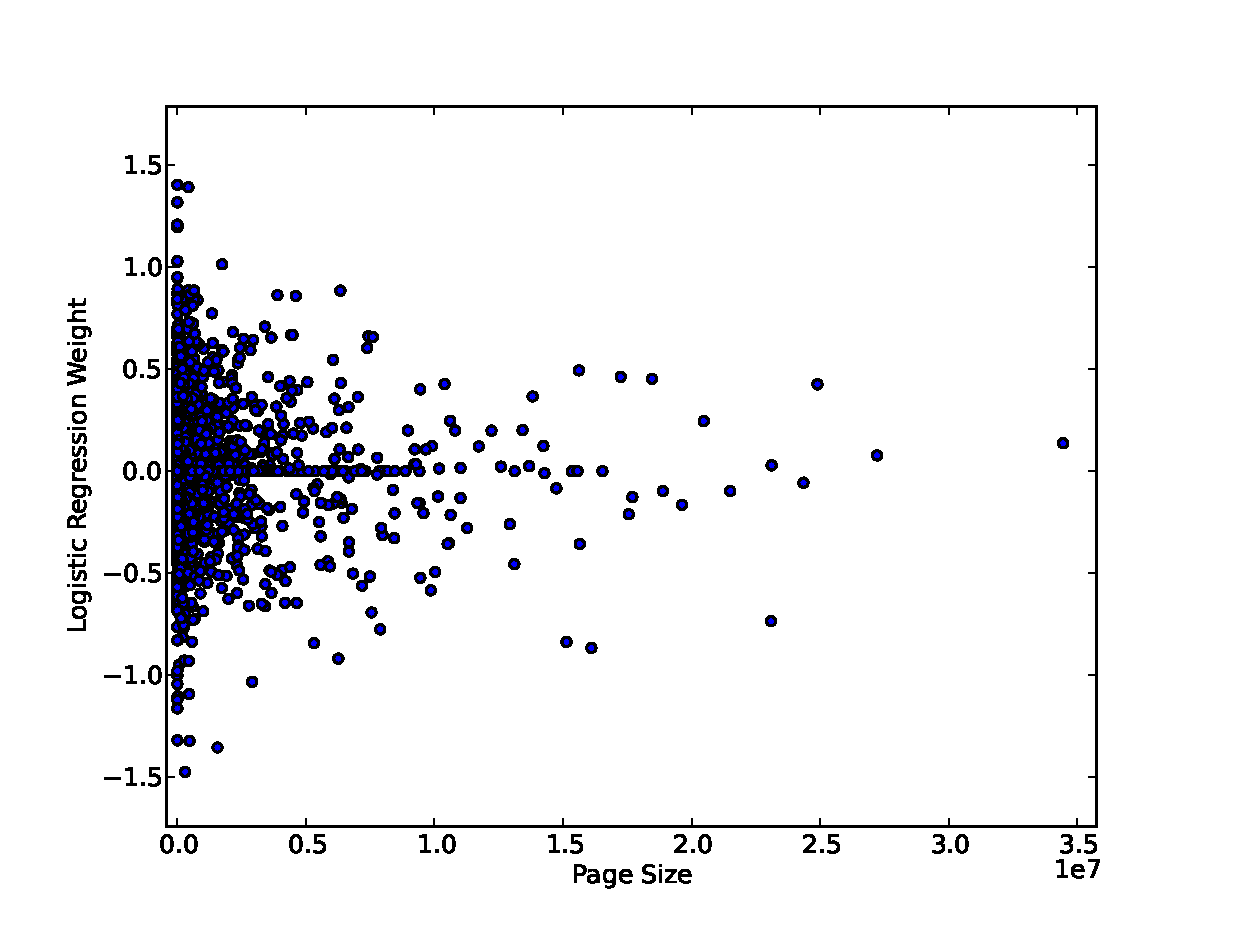
\includegraphics[width=40mm, height=25mm]{data/plots/scatterplots/LRweights/LRweightvsPageSize.eps}}
\subfloat[Fig:][]{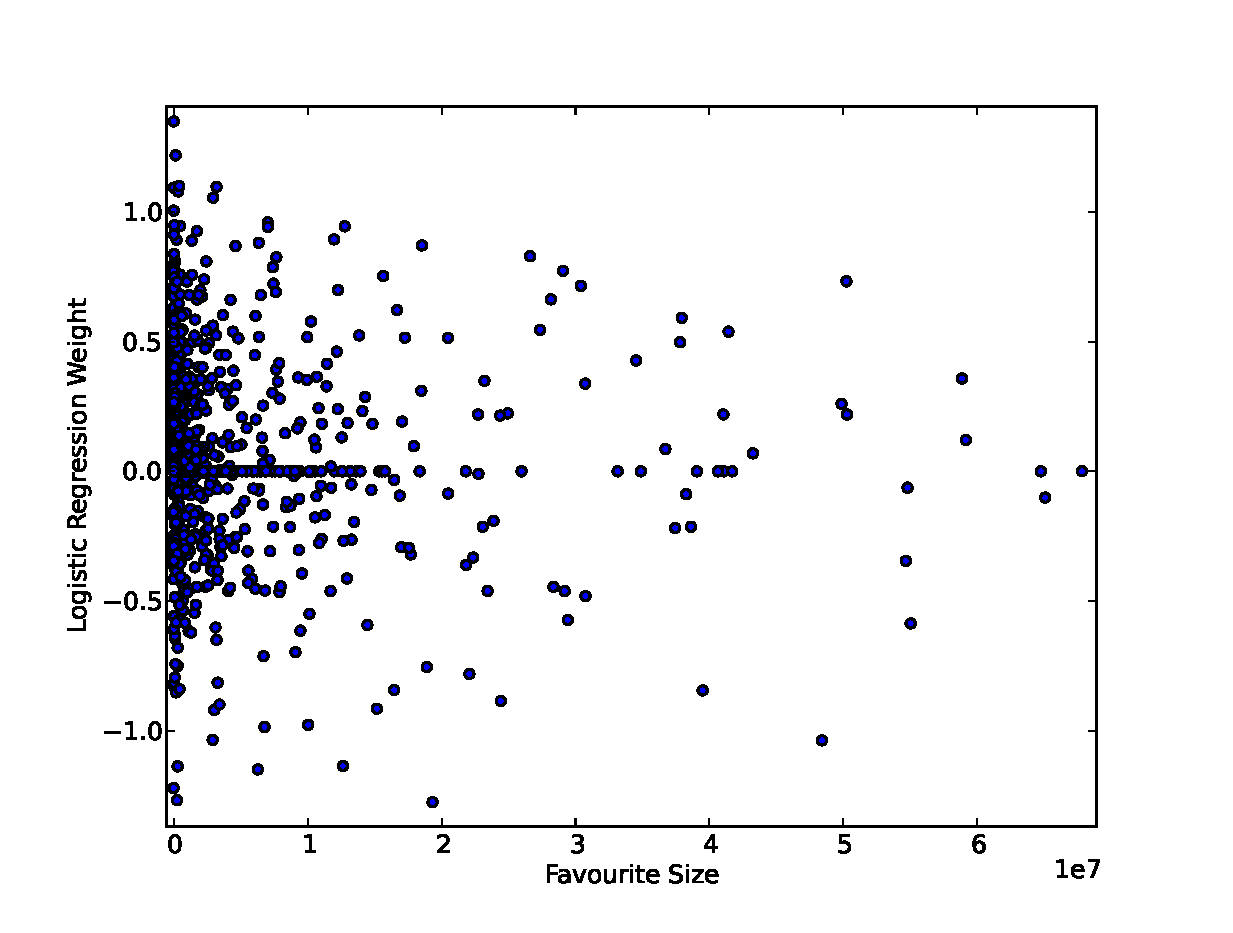
\includegraphics[width=40mm, height=25mm]{data/plots/scatterplots/LRweights/LRweightvsFavouriteSize.eps}} \\
\end{tabular}
\caption {Conditional entropy vs size (a-c); logistic regression feature weights vs size (d-f) }
\label{Fig3}
\end{figure*}

\begin{figure*}[h]
\centering
\begin{tabular}{ccc}
\subfloat[Fig: ][]{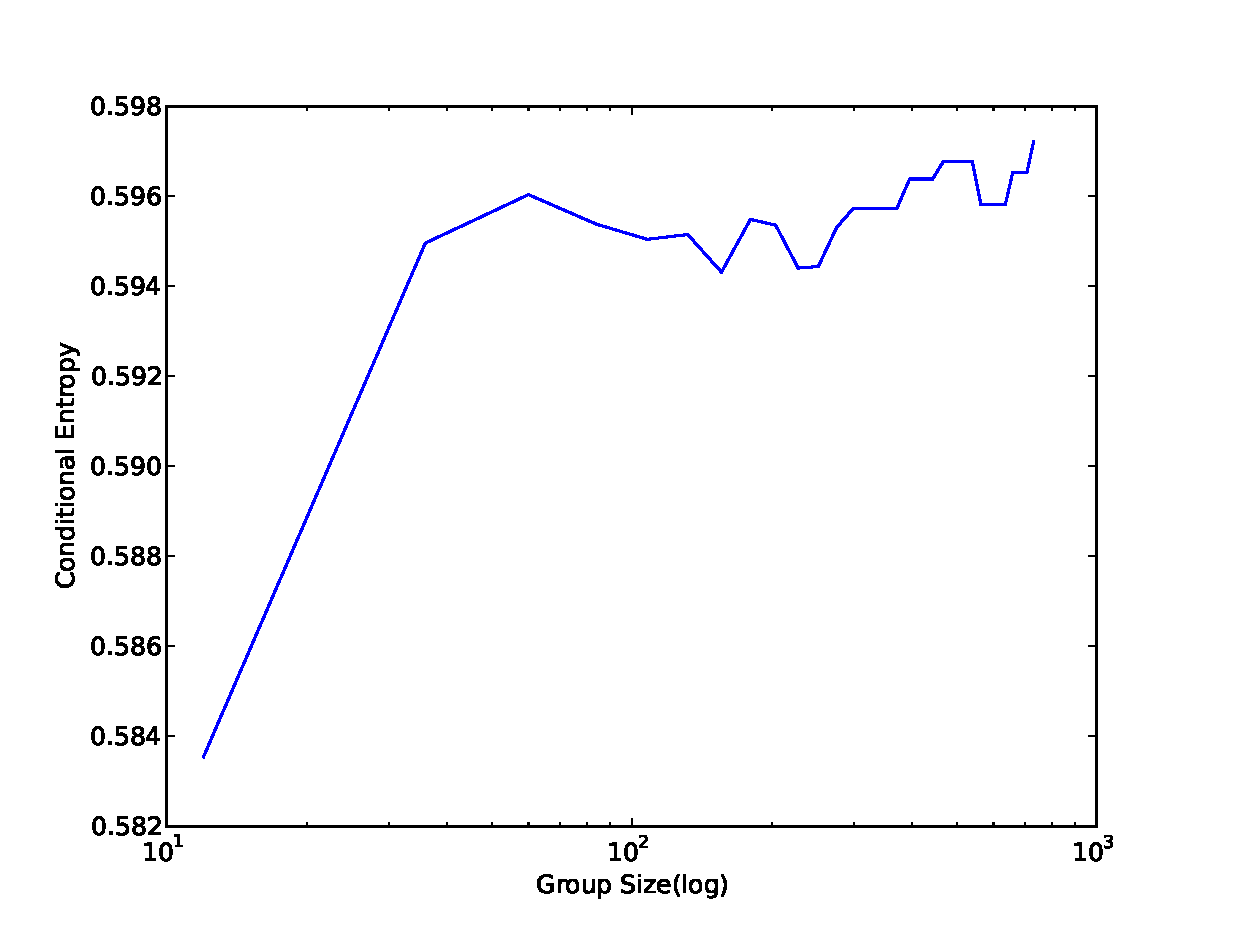
\includegraphics[scale=0.25]{data/plots/cumulativeEntropy/CEvsGroupSize_Top300Features_30bins.eps}}
\subfloat[Fig: ][]{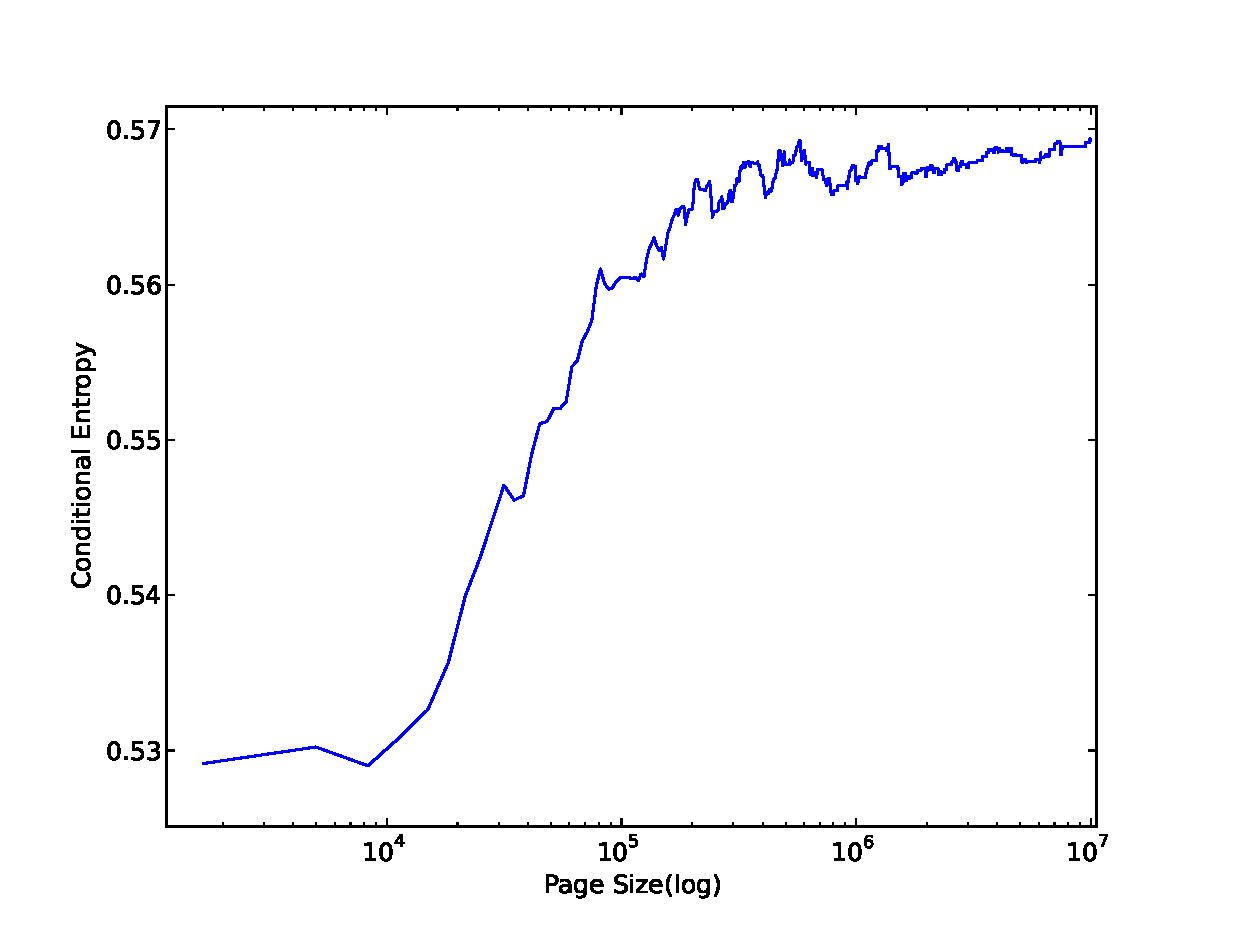
\includegraphics[scale=0.25]{data/plots/cumulativeEntropy/CEvsPageSize_Top800Features_3000bins.eps}}
\subfloat[Fig: ][]{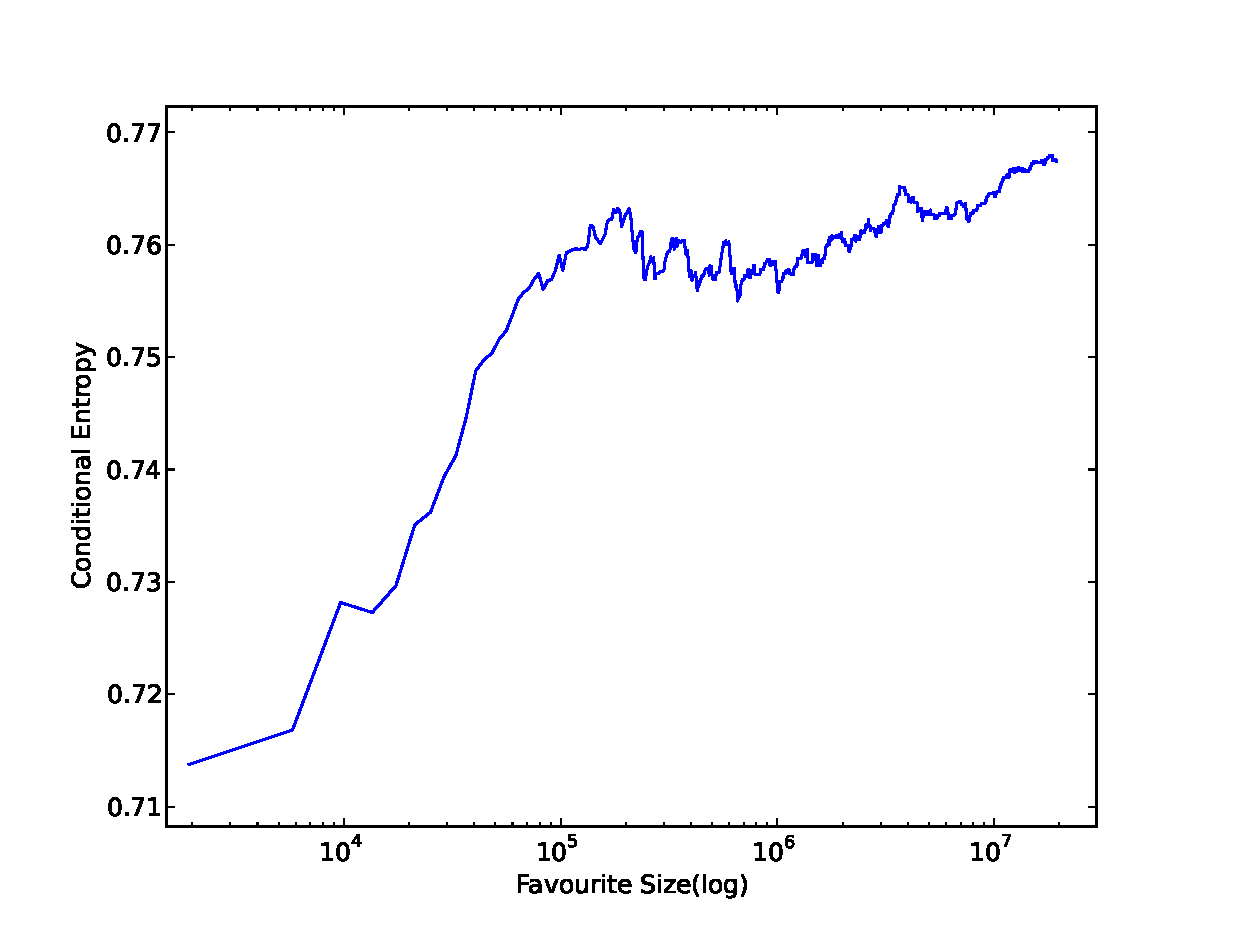
\includegraphics[scale=0.25]{data/plots/cumulativeEntropy/CEvsFavSize_Top800Features_5000bins.eps}}
\end{tabular}
\caption{Average conditional entropy of top 10\% groups, pages and favourites features cumulative over the size }
\label{Fig4}
\end{figure*}

\begin{figure*}
\centering
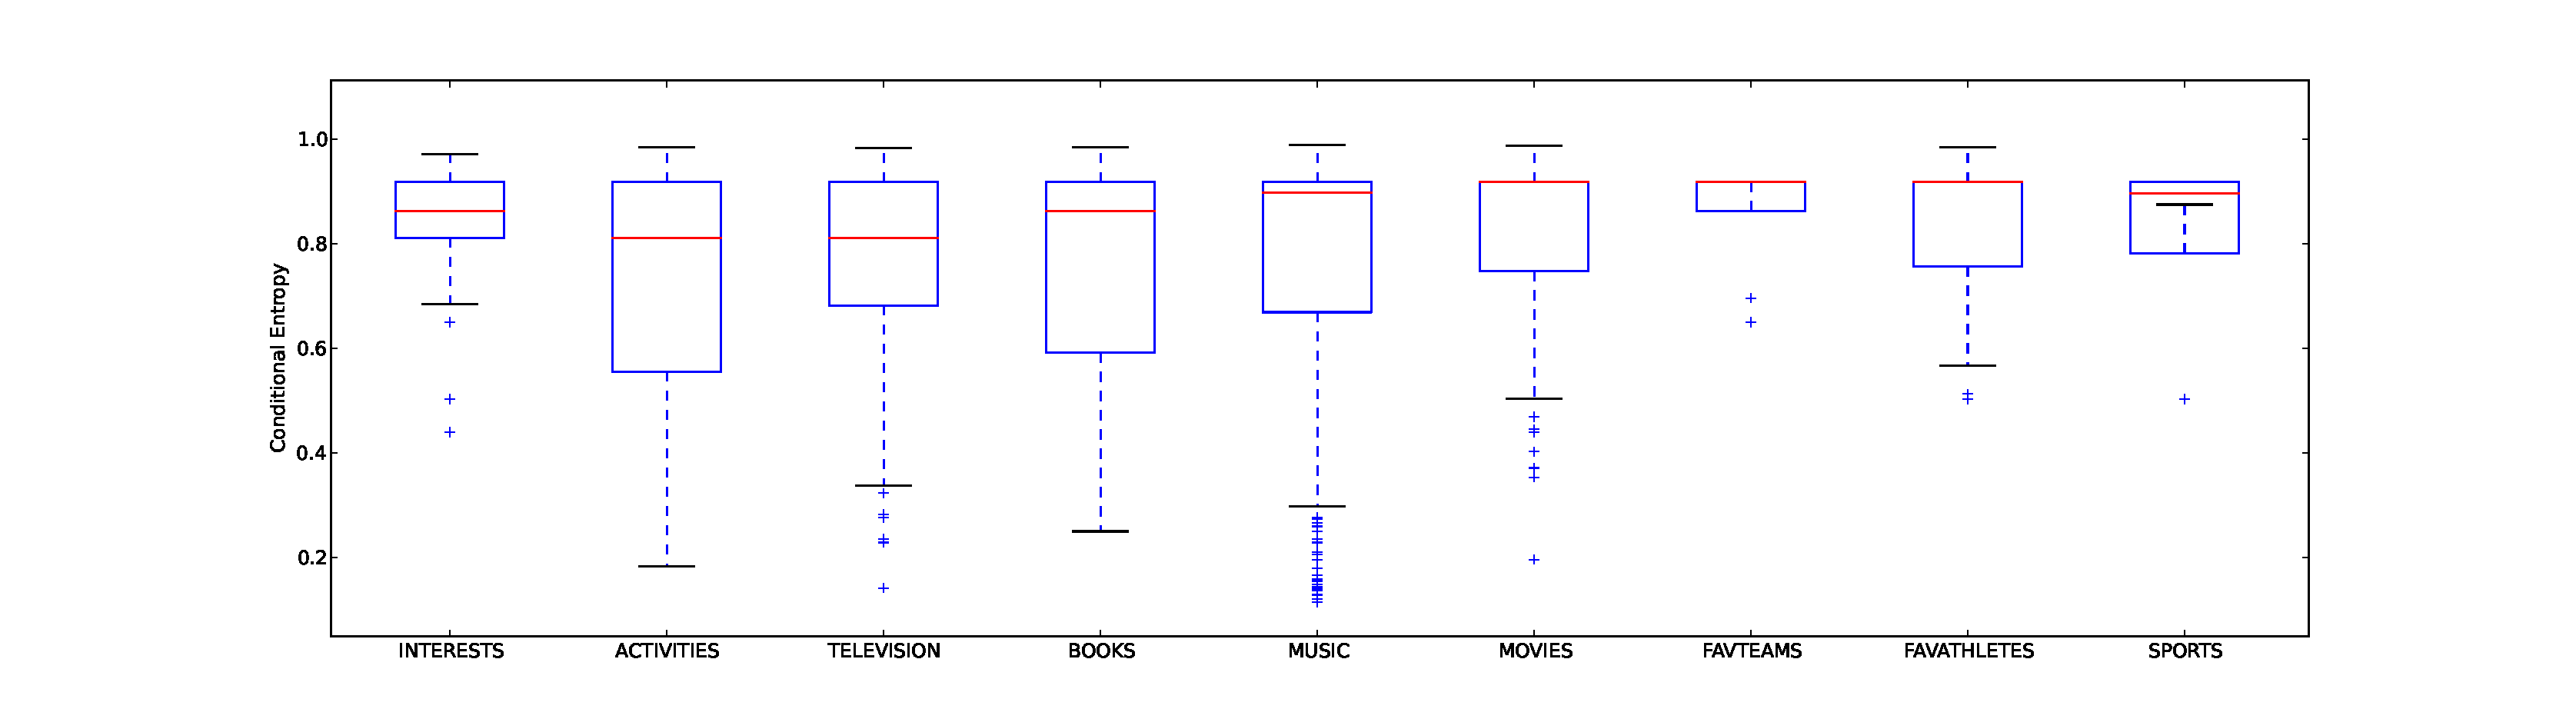
\includegraphics[width=180mm, height=40mm]{data/plots/boxPlots/CEvsFavTypes.eps}
\caption{Conditional entropy for top 1000 favourites breakdown by categories}
\label{Fig5}
\end{figure*}

